\documentclass{standalone}
\usepackage{tikz}
\title{doc}
\begin{document}
	
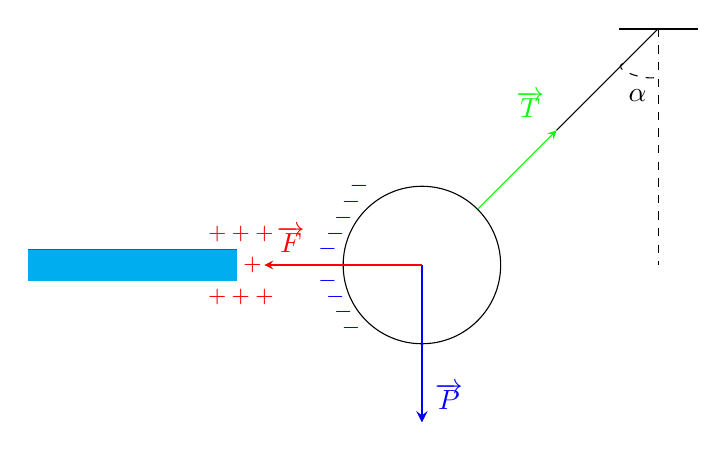
\begin{tikzpicture}
\coordinate (G) at (0, 0);
\draw (G) circle (1);
\draw [-stealth,thick ,  color=blue] (G) -- (0, -2) node[ above right=1pt]{$\overrightarrow{P}$};
\draw [-stealth, color=red] (G) -- (-2, 0) node[ above right=1pt]{$\overrightarrow{F}$};
\draw [-stealth, color=green] (0.71, 0.71) -- (1.71, 1.71) node[ above left=1pt]{$\overrightarrow{T}$};
\draw (1.71, 1.71) -- (3, 3);
\draw [dashed](3,3) -- (3, 0);
\draw [thick] (2.5, 3) -- (3.5, 3);
\draw [dashed](2.56,2.56) to[out=200,in=200] (3.01, 2.39) node[below left=1pt]{$\alpha$};
;
\draw (-2.35, 0.2) -- (-2.35, -0.2) -- (-5, -0.2) -- (-5, 0.2) -- (-2.35, 0.2);
\fill [cyan] (-2.35, 0.2) -- (-2.35, -0.2) -- (-5, -0.2) -- (-5, 0.2) -- (-2.35, 0.2);


\node at (-2,0.4) {\footnotesize\textcolor{red}{$+$}};
\node at (-2.3,0.4) {\footnotesize\textcolor{red}{$+$}};
\node at (-2.6,0.4) {\footnotesize\textcolor{red}{$+$}};
\node at (-2.15,0) {\footnotesize\textcolor{red}{$+$}};
\node at (-2,-0.4) {\footnotesize\textcolor{red}{$+$}};
\node at (-2.3,-0.4) {\footnotesize\textcolor{red}{$+$}};
\node at (-2.6,-0.4) {\footnotesize\textcolor{red}{$+$}};

\node at (-1.1, 0.4) {\footnotesize\textcolor{blue}{$-$}};
\node at (-1.1, -0.4) {\footnotesize\textcolor{blue}{$-$}};
\node at (-1.2, 0.2) {\footnotesize\textcolor{blue}{$-$}};
\node at (-1.2, -0.2) {\footnotesize\textcolor{blue}{$-$}};
\node at (-1, 0.6) {\footnotesize\textcolor{blue}{$-$}};
\node at (-1, -0.6) {\footnotesize\textcolor{blue}{$-$}};
\node at (-0.9, 0.8) {\footnotesize\textcolor{blue}{$-$}};
\node at (-0.9, -0.8) {\footnotesize\textcolor{blue}{$-$}};
\node at (-0.8, 1) {\footnotesize\textcolor{blue}{$-$}};
\node at (-0.8, 1) {\footnotesize\textcolor{blue}{$-$}};


\end{tikzpicture}

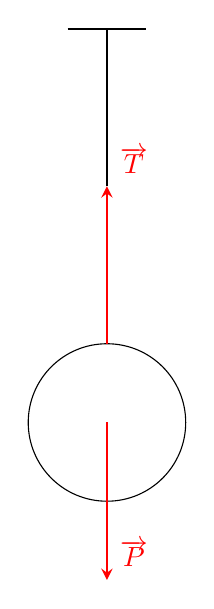
\begin{tikzpicture}
\coordinate (G) at (0, 0);
\draw (G) circle (1);
\draw [-stealth, thick, color=red] (G) -- (0, -2) node[ above right=1pt]{$\overrightarrow{P}$};
\draw (0, 3) -- (0,5);
\draw [-stealth, thick, color=red] (0, 1) -- (0, 3) node[ above right=1pt]{$\overrightarrow{T}$};
\draw [thick] (-0.5, 5) -- (0.5 , 5);

\end{tikzpicture}
\end{document}